\subsection{Carte du jeu}

La carte étant un élément crucial du jeu, au même titre que les mécaniques, 
il m’a semblé important de faire des schémas et de demander l’avis des membres 
du groupe, ainsi que d’autres personnes, afin d’être sûr de mes plans avant de 
commencer. Ainsi, la carte finalement retenue devait avoir suffisamment de 
relief pour rendre les échelles intéressantes, et suffisamment spacieuse pour 
pouvoir la remplir avec au moins 150 personnages non-joueurs (afin de pimenter le jeu).
Dans un premier temps, une forme ronde avait été retenue pour la carte, mais 
a ensuite évolué pour une forme en L, cette dernière rendant l’environnement 
plus naturel et augmentant les chances des personnages de se croiser.


\begin{figure}[hbt!]
    \centering
    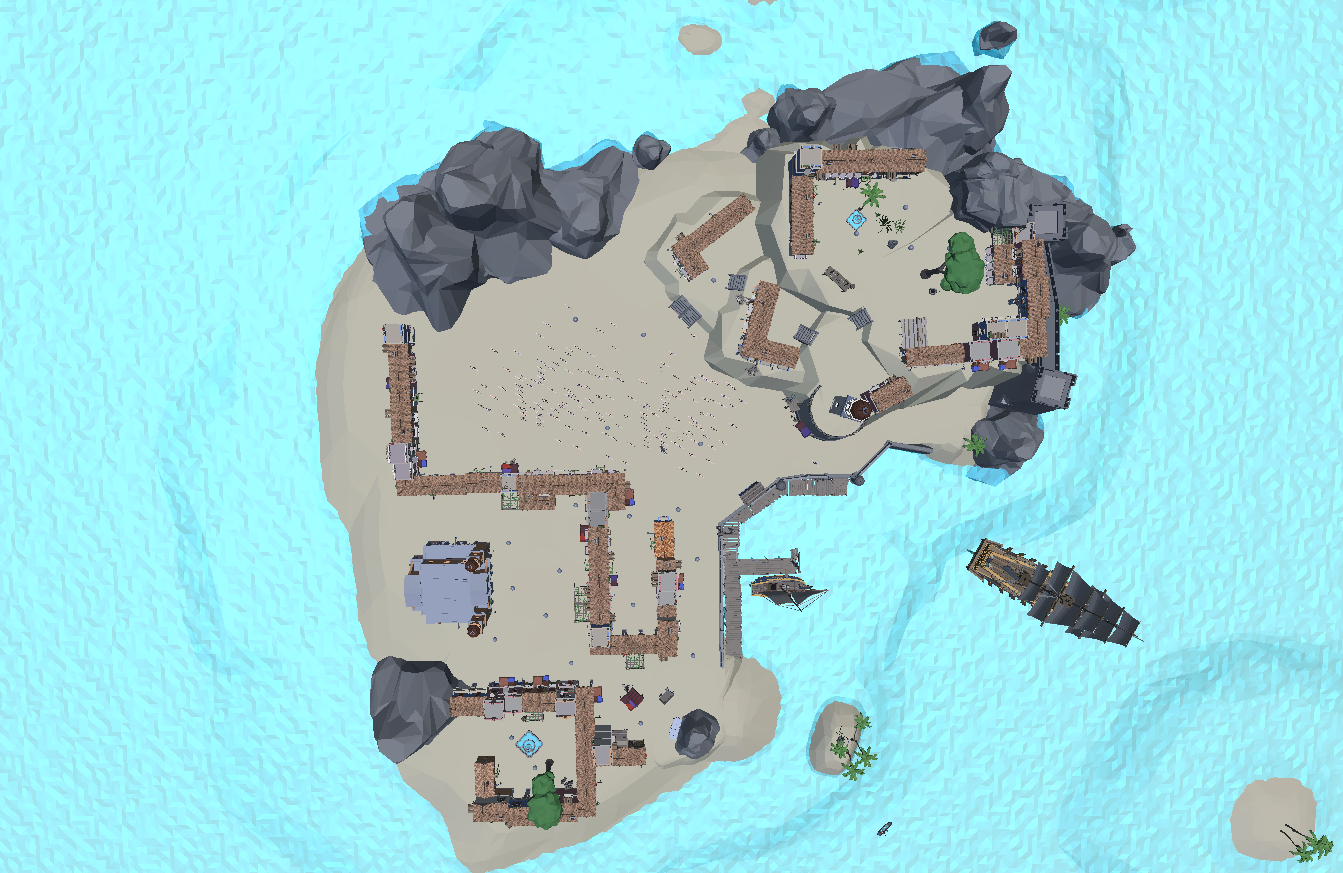
\includegraphics[scale=0.42]{fly_view.png}
    \caption{Vue aérienne de la carte}
\end{figure}

Ensuite, afin d’ajouter du relief à la carte, une colline a été créée. 
Cette dernière s’étend sur environ un quart de la carte, et possède quatre 
niveaux afin d’en permettre l’accès par de petits escaliers successifs. 
Une colline étant un terrain irrégulier, il a été décidé que les bâtiments 
placés sur cette dernière ne seraient pas parallèles, mais répartis afin de 
créer un imbroglio de maisons rappelant le style méditerranéen dont les îles 
comme celle-ci sont inspirées.


\begin{figure}[hbt!]
    \centering
    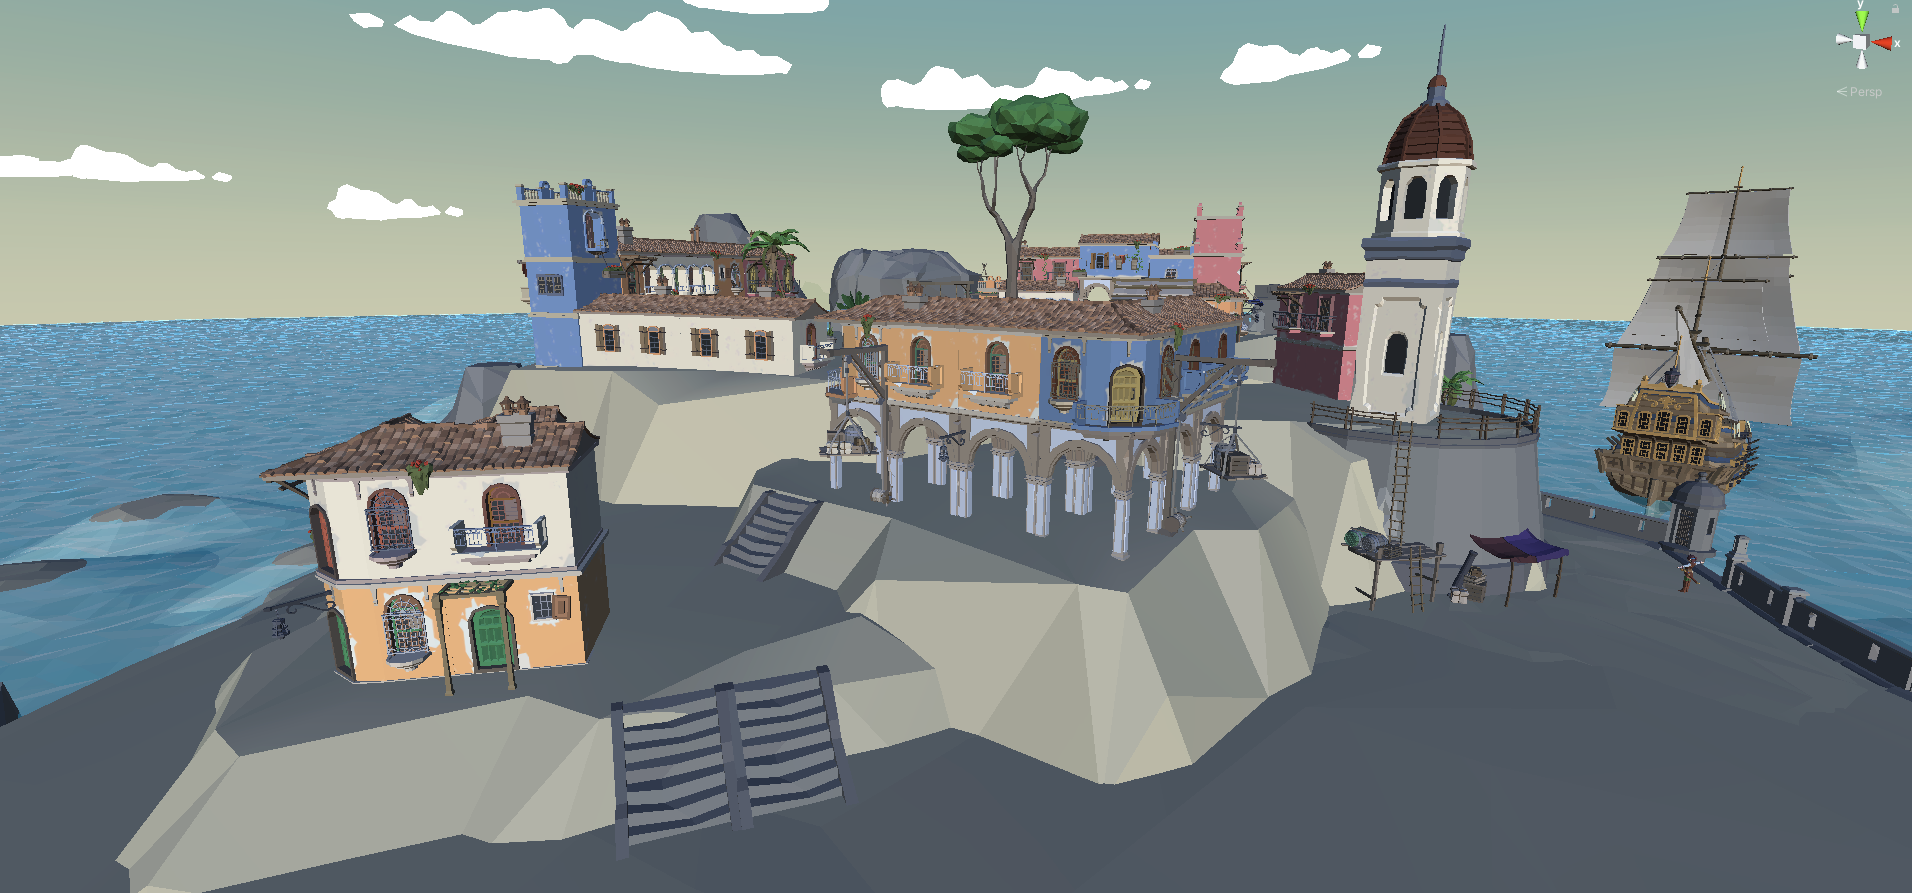
\includegraphics[scale=0.3]{hill.png}
    \caption{Colline de la carte, organisée par étages}
\end{figure}


Enfin, l’architecture de la ville elle-même devant elle aussi avoir une influence 
ibérique, les maisons ont été dessinées basses et organisées autour de places et 
marchés animés. Les tonnelles et les nombreuses lanternes rendent l’environnement 
plus chaleureux, et les arcades, dotées de portes qui se ferment lorsqu’un joueur 
les passe en courant, ajoutent une mécanique de fuite au jeu. L’organisation du 
village se fait autour de la place de l’église, qui fait office de place du marché.\\


Les personnages non-joueurs (NPC) doivent être mus par une intelligence artificielle. 
En outre, ils doivent se déplacer de façon cohérente sur la carte (pas de traversées 
de murs, ni de téléportation par exemple). Le pathfinding intégré à Unity nous a 
donc tout naturellement paru la solution conciliant le mieux efficacité et 
simplicité. Il permet de définir une zone où les NPC peuvent se déplacer, et 
calcule le meilleur itinéraire pour aller d’un point à un autre sans quitter cette zone.


\begin{figure}[hbt!]
    \centering
    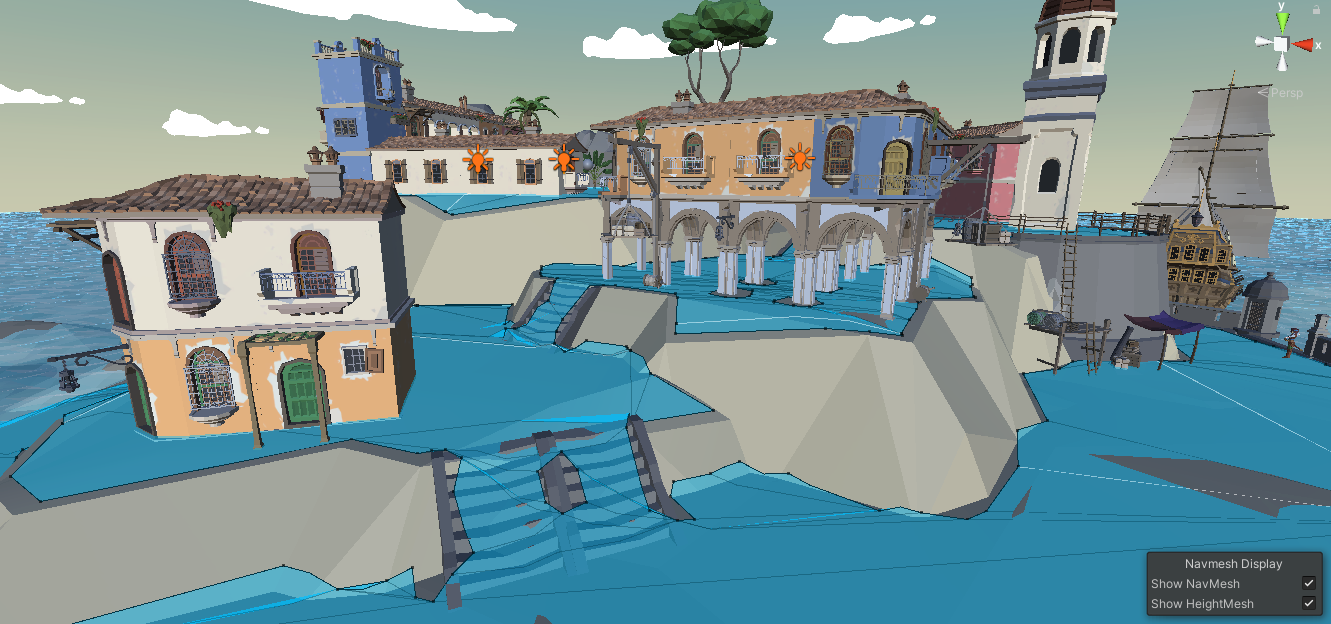
\includegraphics[scale=0.43]{navmesh.png}
    \caption{Le « Navmesh », zone où peuvent se déplacer les NPC}
\end{figure}

L’outil de navigation est assez poussé, et permet de définir les dimensions des 
personnages, ainsi que la hauteur de laquelle ils peuvent sauter et les pentes 
qu’ils peuvent emprunter. Ici, la pente maximale est de 33.4°, mais si ce chiffre 
avait été plus élevé, les pentes sur la capture d’écran seraient devenues bleues, 
et les personnages auraient pu monter sans utiliser les escaliers (ce qui n’est 
évidemment pas le but).
Les joueurs se déplacent donc entre deux points (représentés sur la scène par des 
sphères grises) choisi aléatoirement parmi tous les points de la carte. Un fois 
le point atteint, ils en choisissent un nouveau et s’y rendent. Enfin, si un NPC 
est heurté par un joueur en train de courir, il est étourdi pendant trois secondes, 
puis se relève et repart. \\
Toute cette partie des NPC est déjà fonctionnelle ; cependant l’intelligence très 
limitée de ces derniers pose quelques problèmes, notamment au niveau des escaliers 
où ils se massent et se gênent mutuellement. Il faudra ainsi, dans les prochaines 
versions, améliorer la navigation afin que le chemin emprunté ne soit pas toujours 
le plus court. 

